% Authors' response
\documentclass{scrartcl}
\usepackage[utf8]{inputenc}
\usepackage[english]{babel}
\usepackage{amsmath}
\usepackage{xcolor}
\usepackage{url}
\usepackage{multirow}
\usepackage{graphicx}
\thispagestyle{empty}

\begin{document}
\section*{Authors' response}
To gmd-2019-21 David Simpson (10 Apr 2019):
We apologize for the late response regarding the comments on our paper. We had to evaluate the major concerns raised in the review and found that we have to revise our model and repeat the model experiments to address all concerns. Nevertheless, we will respond to the questions in more detail in the following.

\section{Major points}
\begin{itemize}
\item {\color{blue} Mosaic formulation:}
  \begin{itemize}
  \item {\color{blue} CTM3 claims to implement a mosaic approach, but instead of calculating deposition
rates over each land-cover, and then aggregating using Eqn.3, CTM3 seems to perform the following steps:
\begin{align}
  \label{eq:ra}
  R_a &= \frac{u_z}{u^2_*}\\
  \label{eq:Gsto}
  \overline{Gs^i_g(z)} &= \Sigma^N_{k=1} f_k \times Gs^i_{g,k}(z)\\
  \label{eq:Gns}
  \overline{Gns^i_g(z)} &= \Sigma^N_{k=1} f_k \times Gns^i_{g,k}(z)
\end{align}
As far as I can tell from the text, $R_a$ is calculated once, with the same value of $u_*$ for all land-covers. The CTM3 $R_b$ calculation seems to also use the same $u_*$ over different land-covers, except over sea where a more sophisticated scheme is used. Equations 5-6 above are equivalent to Eqns (22) and (26) from the manuscript. Now I am puzzled however as to how all this is put together. Do they use:
\begin{equation}
  G_c = \mathrm{LAI} \cdot \overline{Gs^i_g(z)} + \overline{Gns^i_g(z)}
\end{equation}
  }
    The referee is correct regarding the usage of Eq.~(\ref{eq:ra}) and Eq.~(\ref{eq:Gns}). In case of stomatal conductance, we first compute:
    \begin{equation}
       \overline{gs^i_g(z)} = \Sigma^N_{k=1} f_k \times gs^i_{g,k}(z).
    \end{equation}
    This is put together as follows:
    \begin{equation}
      \label{eq:Gsto_corr}
      G_c = \mathrm{LAI} \cdot \overline{gs^i_g(z)} + \overline{Gns^i_g(z)}
    \end{equation}
  \item {\color{blue} In any case, I think this approach has serious problems. Why average first for $G_s$ and then for $G_{ns}$ , when it is the fluxes ($F_k$ , or $V^i_{g,k}(z_\mathrm{ref}) \times \chi^i_\mathrm{avg}(z_\mathrm{ref})$) which need to be averaged? I also do not understand why they would use the same $u_*$ and $R_a$ for all land-covers. I think the authors need to make a case for their approach, or change it.}
    Thank you very much for your detailed account of the \emph{mosaic approach}. We have discussed the concerns raised within this comment and found that we have indeed made a mistake in our implementation of the \emph{mosaic approach} which forces us to revise our model and repeat the model experiments.
  \end{itemize}
\item {\color{blue} Calculation of $R_a$:}
  \begin{itemize}
  \item {\color{blue} $R_a$ in CTM3 appears to be calculated just once, and from a height of 8\,m. This means
that there is no consistency between the $R_a$ term and the underlying surface, which is
clearly wrong. The similarity equation for $R_a$ given in their Eqn~(2) is very standard and has been
used for decades (Garratt 1992). As pointed out by Ref~1, the equation as given has
errors. The correct equation will not give negative values unless presented with wrong
inputs, and I suspect that that is what has happened.}
We have, in fact, not presented "wrong inputs" to the algorithm.
As pointed out by Ref \#1, Eq. (2) in our manuscript is erroneous. We have not only made a mistake when deriving the formulation for $R_a$, from $u_*$ as presented in S2012 (sign-flip preceding the last term in the series) but also mistype the denominator of the second term. The corrected equation:
\begin{equation}
  R_a = \frac{1}{\kappa u_*}\left[{\ln{\left(\frac{z-d}{z_0}\right)}-\Psi_m\left(\frac{z-d}{L}\right)+\Psi_m\left(\frac{z_0}{L}\right)}\right].
  \label{eq:aero_res}
\end{equation}


\item {\color{blue} It is actually difficult to tell what
was tested from the manuscript though, since they state simply that $d$ is ’typically 0.7\,m’.
Did they use $d$ properly, consistent with the underlying land-cover and its $z_0$? Did
they assume that their 8\,m meteorology was at a physical height of 8\,m, or at $d + 8\,\mathrm{m}$.
If the latter, which $d$?}
  It is indeed not clear from the manuscript that we never actually implemented the formula (Eq.~(2) in our manuscript) in the model. The reason for this were simple, mathematical considerations. Given $z = z_\mathrm{ref} = 8\,\mathrm{m}$ and $d = 0.7\cdot 1\,\mathrm{m}$, we looked at certain parameter spaces for $L$ and $z_0$ (e.g., $0 \le z_0 \le 2.5$ for vegetated land surfaces from a climatology mean derived from ISLSCP2 FASIR) but have not taken the consistency "with the underlying land-cover and its $z_0$" into account (see Fig.~\ref{fig:test_ra}). This might have been not unsophisticated enough, though. The statement "$d$ is ’typically 0.7\,m’" is a typo and should of cause be corrected to \emph{typically $d = 0.7\cdot h(N,\mathrm{lat})\,\mathrm{m}$ for vegetation other than forests}. Note: The average height of the lowermost model level is actually $20\,\mathrm{m}$ ($10\,\mathrm{m}$ for mid-level).
  
  \begin{figure}
    \centering
    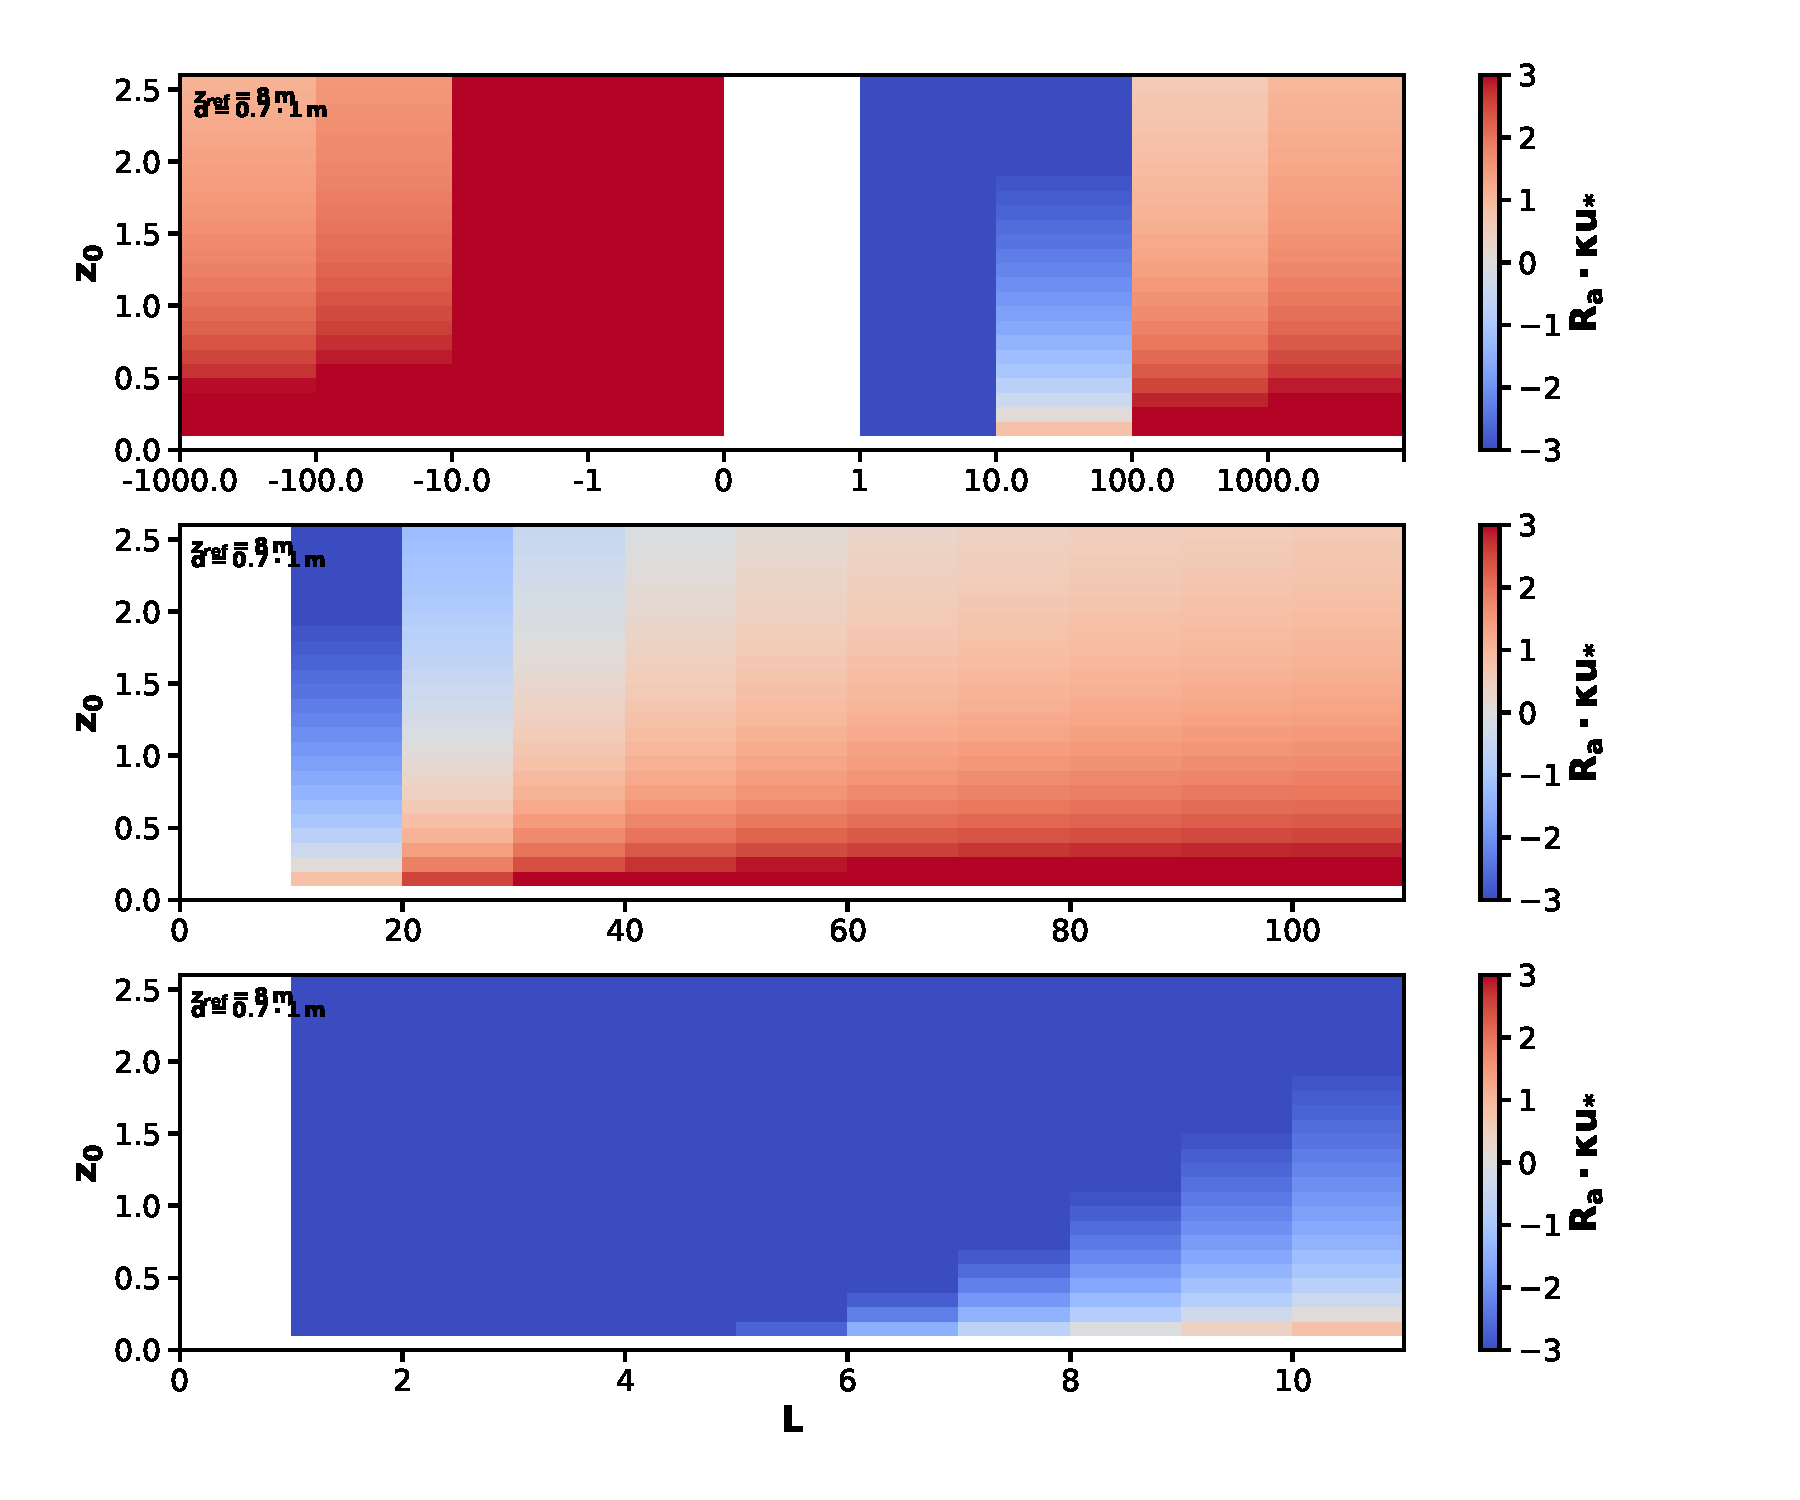
\includegraphics[width=0.8\textwidth]{test_Ra_wrong_form.pdf}
    \caption{Test cases for $R_a$ with $z = z_{ref} = 8\,\mathrm{m}$ and $d = 0.7\cdot 1\,\mathrm{m}$.}
    \label{fig:test_ra}
  \end{figure} 

\item {\color{blue} Lines 19--30 of this section explain the Monteith alternative, but in a rather confusing
way. For example, when is $z_0$ ever zero, as stated on line 23, or why does $\partial_z R_a \rightarrow R_a $
for finite $z$? (I know what they intend to say, but it isn’t at all clear.)}
  The referee is right. The text and derivation of the Monteith relation is confusing. We will elaborate on this in a revised version of the manuscript in case we are not going to use Eq.~(\ref{eq:aero_res}).

\item {\color{blue} In any case, here
the authors end up with a stability-independent equation for $R_a$, without mentioning or
discussing that fact.}
  We shall elaborate on this.
\item {\color{blue} This very shallow layer is also very problematic for deposition calculations in general,
since the model cell seems to be run here with horizontal dimensions of $2.25 \times 2.25^\circ$,
or about $250 \times 250\,\mathrm{km}$ near the equator, but a vertical mid-level (CTM3’s $z_\mathrm{ref}$) of
just 8\,m. Now, profiles of wind and depositing gases are very sensitive to the underlying
surface, and should be very different for forests or lakes for example. Any wind-speed
or friction velocity calculated from a model of such large horizontal resolution will necessarily give values
at 8\,m which reflect the whole grid. Deposition rates for a specific
land-cover will vary enormously depending on what else is in the grid-square. (Although not strictly comparable,
we showed in Schwede et al. (2018) that differences
between the grid-average and forest specific deposition rates of N-compounds could be
as much as a factor of two and up to more than a factor of five in extreme cases. These
differences were largely dependent on how much forest occupied each grid cell.)}
  In S2012, $R_a$ is evaluated "at around $45\,\mathrm{m}$" which is similar to the center of our second lowest model level. We can easily correct for this in a revised model version. 
\end{itemize}      
\item {\color{blue} Why so much focus on sea areas?: The text seems rather unbalanced with regard to the different land-covers. Sect. 2 uses 1/2 page on various $z_0$ corrections for oceans, but say nothing about the ecosystem
where ozone is expected to deposit at high rates: forests, crops, and other terrestrial
ecosystems. The supplementary has three Figs related to this oceanic deposition. Why?}
  The referee is right that ozone is predominately deposited to terrestrial ecosystems, which cover about 2/9 of the Earth's surface, while 2/3 is covered by oceans. Nevertheless, due to the ocean's vastness, relatively small changes in modeled dry deposition easily accumulate and influence the atmospheric ozone concentration. Luhar et al. (2017, 2018) show that the current models may overestimate the oceanic ozone sink by a factor of three -- rendering the ocean a even smaller sink for ozone.
  
  This said, Section~2 as a whole consists of about 9 pages, of which 1/2 page is dedicated to oceans ($R_b$ computation) and 7 pages are dedicated to vegetation especially stomatal and non-stomatal conductance ($R_c$ computation). Hence, we do not see a significant unbalance in favor of oceans herein.

  Regarding the three figures with respect to ocean in the supplementary material: The reason for these is that we found the "legacy code" in the model (linear fit dynamic viscosity of air $\mu(T)$) after we had finished the implementation of the new dry deposition scheme, run the experiments, and done the analysis on these. We had to verify that this had no influence on the results. 
  
\item {\color{blue} Use of the term 'EMEP scheme'?: Sect. 3 discusses the comparisons of $V_g$ in terms of ’EMEP scheme’ versus
  ’Wesely scheme’, and sensitivity tests are named e.g. ’EMEP\_offlight’. As noted above
the scheme implemented in CTM3 is very different to that implemented in the EMEP
model, so this is very misleading. Please rename your scheme to something else.
I am worried that readers might get the impression that it is the EMEP scheme which
is being tested here, but it certainly is not. [...]}
  We apologize for the misleading naming of the new dry deposition scheme in the Oslo~CTM3 which is (partly) based on the formulations in the publication the referee refers to as \emph{S2012}. By no means have we meant to offend any of the original authors of the EMEP/MSC-W model nor intended to misguide the readers. We will rename the revised scheme appropriately ($\rightarrow$\emph{mOSaic scheme}). 
\item {\color{blue} Reproduction of material from S2012:}
  \begin{itemize}
  \item {\color{blue} As far as I can see, Table S1, S2 and S3 are taken directly from S2012, with no change to parameters. It is not usual to copy tables from the work of other authors in this way.
    Just refer to S2012 (and give Table number as help).}
    We will follow this advice and refer to the tables in S2012 accordingly.
  \item {\color{blue} Many of the equations are from S2012, and many not. I would like the authors to
    make this very explicit, so that readers are not confused as to what comes from EMEP,
    and what has changed for CTM3.}
    We are going to elaborate on this matter in a revised version and point out our equations' sources more clearly.
  \end{itemize}
\end{itemize}
\section{Minor points}
\begin{itemize}
\item {\color{blue}P1 L22. Isn’t $\mathrm{H_2O}$ the most important greenhouse gas? (Say anthropogenic
  GHG perhaps?)}
  Thank you for pointing this out. We follow the advice and write: \emph{"[...] ozone is a potent anthropogenic greenhouse gas [...]"}
\item {\color{blue}P2 L3. The Wilson ref only concerns Europe, and its focus on the 95th percentile can hide trends
  found at higher percentiles (e.g. Simpson et al. 2014). A better ref would be Fleming et al. (2018) or Mills et al. (2018a). By the way, the most recent calculation on food security (using flux approaches) is now Mills et al. (2018b).}
  Thank you for pointing out these new publications. We take them into consideration, when revising the manuscript.
\item {\color{blue}P2 L11. What does in situ mean here? Ozone production can take place over
  days of transport.}
  \emph{In situ} typically means \emph{on site, locally}. In this context, we use it exactly in this meaning. Elevated ozone levels at a site originate mainly from the local production of ozone from its precurors that are transported than from advection of ozone itself. Although long-range ozone transport occures and might be most important in regions that else lack precursors. We elaborate on this in a revised version of the paper: \emph{Tropospheric ozone is mainly produced locally [...] involving advected precursor gases [...]}
\item {\color{blue}P2 L25--35. This text about halogens is not really relevant to a dry deposition
paper. Reactions with bromine can be important sinks, but are not usually counted
as deposition.}
  The removal of ozone from the Arctic boundary layer in the precence of halogens is indeed not directly related to ozone dry deposition, but one of the discussed mechanisms to trigger the bromine explosions involves, e.g., a "initialisation" by ozone dry deposition. But we see that this is of no relevance to ozone dry deposition itself, but to the observed ozone abundances in the Arctics. We may remove these reference in the revised version of the manuscript.
  
\item {\color{blue}P3 L2--3. Why specify mid-June maximum for ozone. Monks (2000) might
  take issue with that, as would for example Sinha et al. (2015).}
  The referee has got a point here. Of cause the maximum of ozone in the annual cycle depends on the location. We remove this specification.
\item {\color{blue}P3 L4--5. There are plenty of ozone measurements made outside Europe. The
authors appear to be unaware of the massive ozone collections made under the
TOAR project (see e.g. Flemming, Mills refs below), or the high quality data
available from GAW (inha 2015).}
  Thank you for reminding us of the data collected under the TOAR project. We knew about this dataset but have to admitt that we have not made much use of it, yet. We have, however, not stated that there are, in general, no sites outside of Europe, but that long-term obersvations (started before the 1950s) are only found in Europe. Maybe the term "long-term" is not clear enough. We add: \emph{"[...] a limited number of long-term ozone observations (started before the 1950s)[...]"}
  
\item {\color{blue}P3 L16. One also has dry deposition to water, as this paper makes clear later on.}
  That is indeed true, but we didn't want to name all possible surfaces onto which dry deposition takes place. We, hence, shall write: \emph{"Removal of any substance from the atmosphere which is not involving rain, e.g., through gravitational settling or by uptake by plants and soil, is referred to as dry deposition.}
  
\item {\color{blue}P3 L20. One usually refers to dry deposition as something between a near-
surface height (e.g. z = 1m, 10m, or 50m) and the surface, not from $z_0$. In fact,
at $z = z_0$ one has $u_z = 0$, and hence the author’s $R_a$ just below should be zero.}
Thank you for pointing out this inaccuracy. We, of cause, meant "near-surface" height or lowermost model level (which is indeed not at $z_0=0$). We change the text accordingly: \emph{"[...] dry deposition is a product between near-surface ozone concentration $\mathrm{[O_3](z_0)}$ (e.g. the lowermost model level) [...] "}
  
\item {\color{blue}P4 L20. I would remove the term textbook knowledge, since there are many
different approaches to nearly all these equations. It is thus good that the equations
as used in CTM3 are spelled out explicitly.}
  We follow the advice and remove the sentence in which the term occurs and write: \emph{"[...] we will give a detailed account of the new dry deposition scheme and the equations that we use."}
  
\item {\color{blue}P5 L5. I would add Emberson et al. (2000a) and Tuovinen et al. (2004) to
the list of EMEP refs here, since this was the first publication of the methods that
have more or less been used until today.}
  We have added the references regarding the EMEP MSC-W model. \emph{"[...] we follow the European Monitoring and Evaluation Programme (EMEP) MSC-W model (Emberson et al., 2000; Simpson et al., 2003; Tuovinen et al., 2004; Simpson et al., 2012), [...]"}
  
\item {\color{blue}P7, notation. In S2012 and EMEP generally, we use upper-case G and R to refer
to canopy-scale (bulk) variables, and lower-case for leaf-scale. Thus, in EMEP
we would have $G_\mathrm{sto} = LAI g_\mathrm{sto}$. Here the authors seem to mix upper and lower
case between their equations (13) and (14).}
  This is probably related to the referee's major point 1. Since our approach, averaging the resistances/conductances instead of the fluxes, is incorrect, this part of the manuscript has to be revised in any case. But to answer the question: Eq.~(13) should have been placed at the end of the section, after the definition of $G_\mathrm{sto}$ and $G_\mathrm{ns}$. A better notation is found Eq.~(\ref{eq:Gsto_corr}). We shall also go through all our notations in that section to make it more comprehensible.
  
\item {\color{blue}P7 Eqn (13). Is LAI one-sided, 2-sided, projected .... define.}
  LAI is one-sided taken from ISLSCP2 FASIR. We add this to the sentence: \emph{"[...] $\text{LAI}$ is the one-sided leaf area index taken from ISLSCP2 FASIR [...]"}
  
\item {\color{blue}P8 L1. S2012 do not suggest using depths lower than 1\,m. We use SMI3 which
  is from 28-100 cm.}
Thank you for the clarification. We might have mixed this up. Since we have to repeat our simulations, we will choose SWLV3 from the start.
  
\item {\color{blue}P8 L2. Why did you choose to use the surface (0--7\,cm) soil moisture?}
  The reason for the initial choice of 0--7\,cm came from the project this work is related to. In our project, we are interested in ozone in boreal regions where the soil column is generally more shallow. 
  
\item {\color{blue}P8 L18. This is wrong. Nothing in the EMEP model is used to ’mimic the
time lag..’. We use the light function to modify stomatal conductance, as with the
other $f$ factors.}
  We change this inadequate formulation: \emph{"[...] this integrated photon flux is used to modify the stomatal conductance in response to light."}
  
\item {\color{blue}P9 L20, and Table 1. The consequence of Table 1 is that vegetation at $0.5^\circ\,\mathrm{N}$
will start growing at day 90, whereas those at $0.5^\circ\,\mathrm{S}$ will start on day 272. (By the
way, in EMEP now we use monthly factors from the LPJ-GUESS model to derive
phenology for non-European areas, because of such difficulties with tabulations.)}
  Thank you for the remark. We see this problem. Using an actual land model would solve this, but at that point it is not feasible to integrate such in the Oslo~CTM3.
  
\item {\color{blue}P9 L18. what do you mean by "surface or 2\,m"? Surface might refer to skin or
  leaf temperature?}
  
\item {\color{blue}P9 Eqn (26). Say 1st and 2nd, not I. and II.}
  We may change Table~1 accordingly.
  
\item {\color{blue}P9, Eqn (27). This equation is a modification of Erisman’s original (1994) formulation, so explain that.}
\item {\color{blue}P10 L12. Be explicit that this statement refers to S2012. The current EMEP
model uses different heights for e.g. tropical vegetation.}
\item {\color{blue}P11 Sect 2.2. I also found this aerosol section confusing. Eqn (30) is from S2012,
and so is the factor 0.008.SAI/10 used in Eqn (33), but here new a 1 coefficients
are defined. Did the ’aerosol microphysic model’ referred to also mix equations
in this way? Is there any publication as to the reliability of this method?}
\item {\color{blue}P12 Fig.2. I didn’t understand what is being done here. The Figure suggests that
the EMEP scheme has one category for ’Forests, Med. scrub’, whereas S2012
lists 4 types of forest, as well as Mediterranean scrub as a separate ecosystem.
This figure also suggests that EMEP has savanna, which it doesn’t, but do have
many other categories (Table 3 of S2012 lists 16 main categories. The current
EMEP model has 32.)}
\item {\color{blue}P12 L13. Again, the current EMEP model is not eurocentric, and uses global
phenology calculations.}
\item {\color{blue}P13 Sect 2.3.2. The initial lines (14-16) are hard to understand and only by
reading further do I see what they mean by ’de-accumulated’. If working with
IFS PPFD is so hard, why didn’t the authors just calculate hourly (or minute-by-
minute) PPFD using cloud-cover and zenith angles?}

\end{itemize}
\newpage

\end{document}
